% ******************************* Thesis Appendix C ********************************

\chapter{Modelsim Simulations}
\label{appendix:2}
\section{Simulations with 10 Observer}
\begin{figure}[h]
\centering
%\hspace{3.0cm}
%\vspace{-5cm}
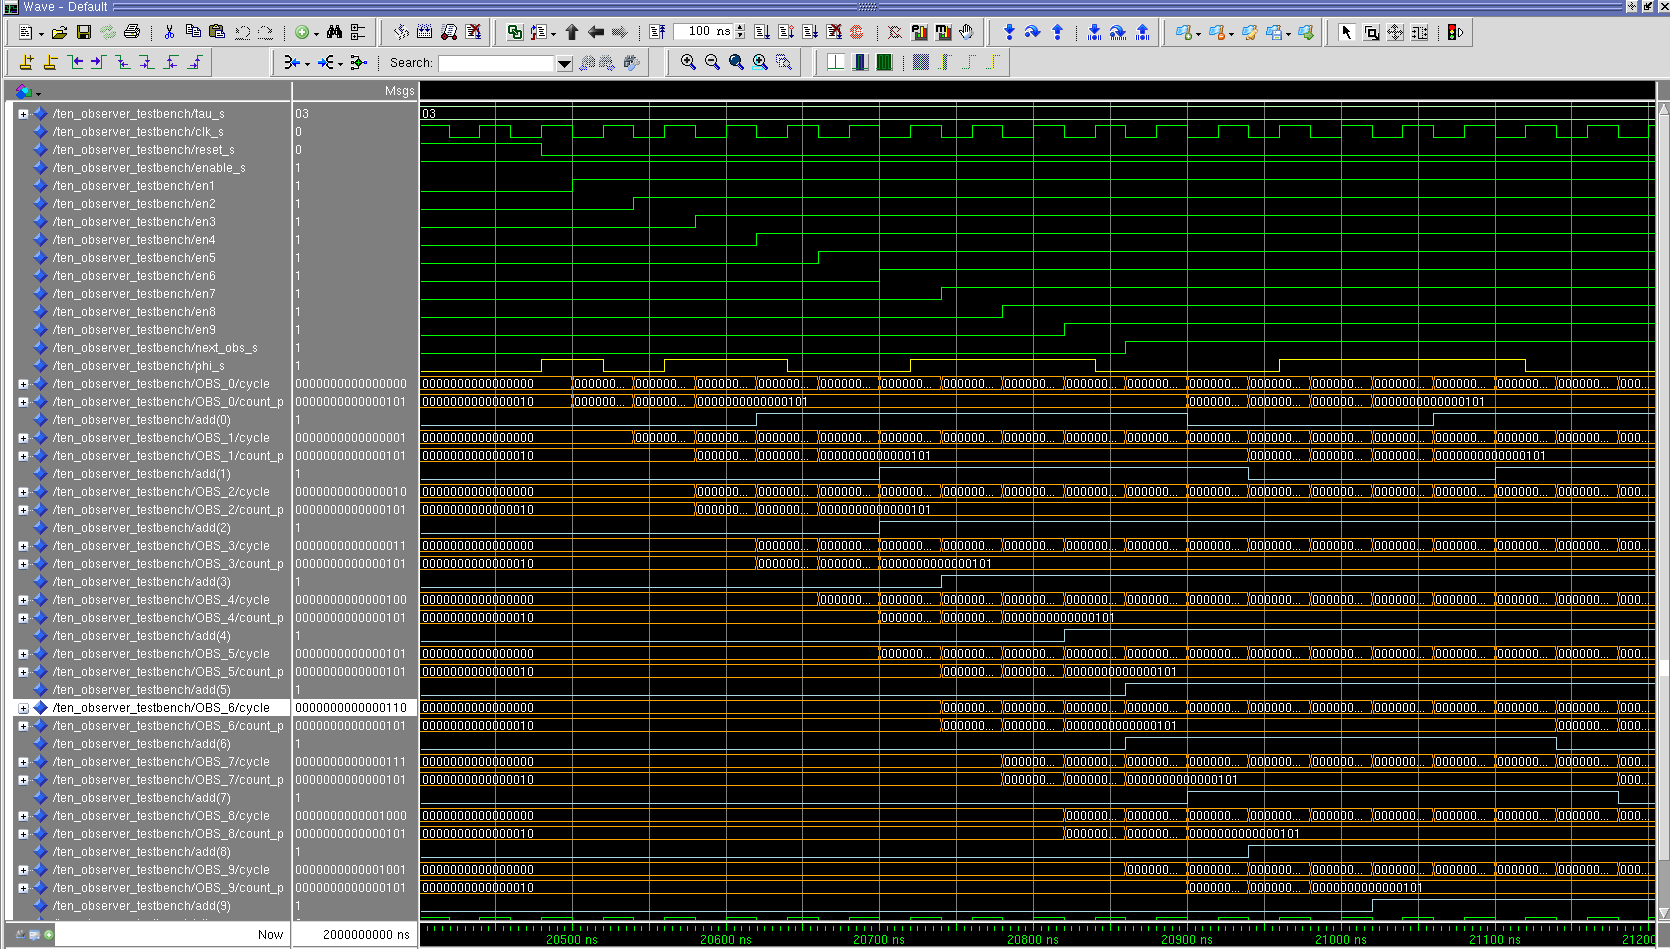
\includegraphics[width=650px,height=300px,angle=-90]{../../pictures/Modelsim/10_Observer_tb_1.png}
%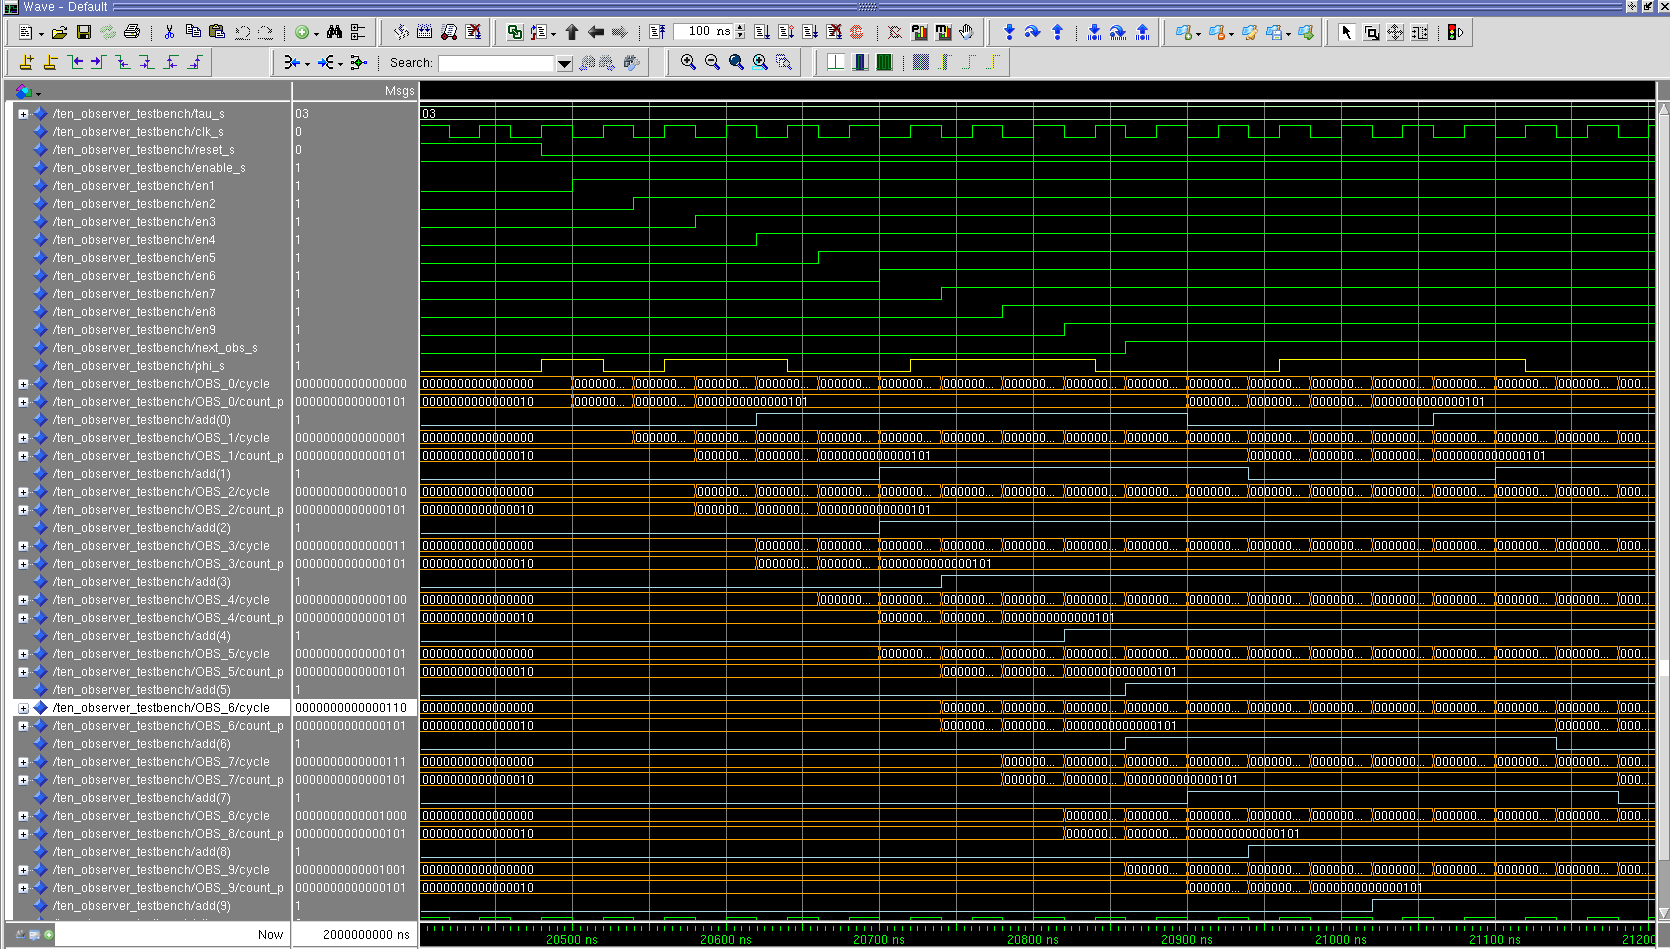
\includegraphics[height]{../../pictures/Modelsim/10_Observer_tb_1.png}
\caption[Modelsim Simulation of 10 Observer - 1]{m=10 Observer and $\tau=3$ with view about cascade activation of the observer}
\label{fig:simulation:ten:first}
\end{figure}

\begin{figure}[h]
\centering
%\hspace{3.0cm}
%\vspace{-5cm}
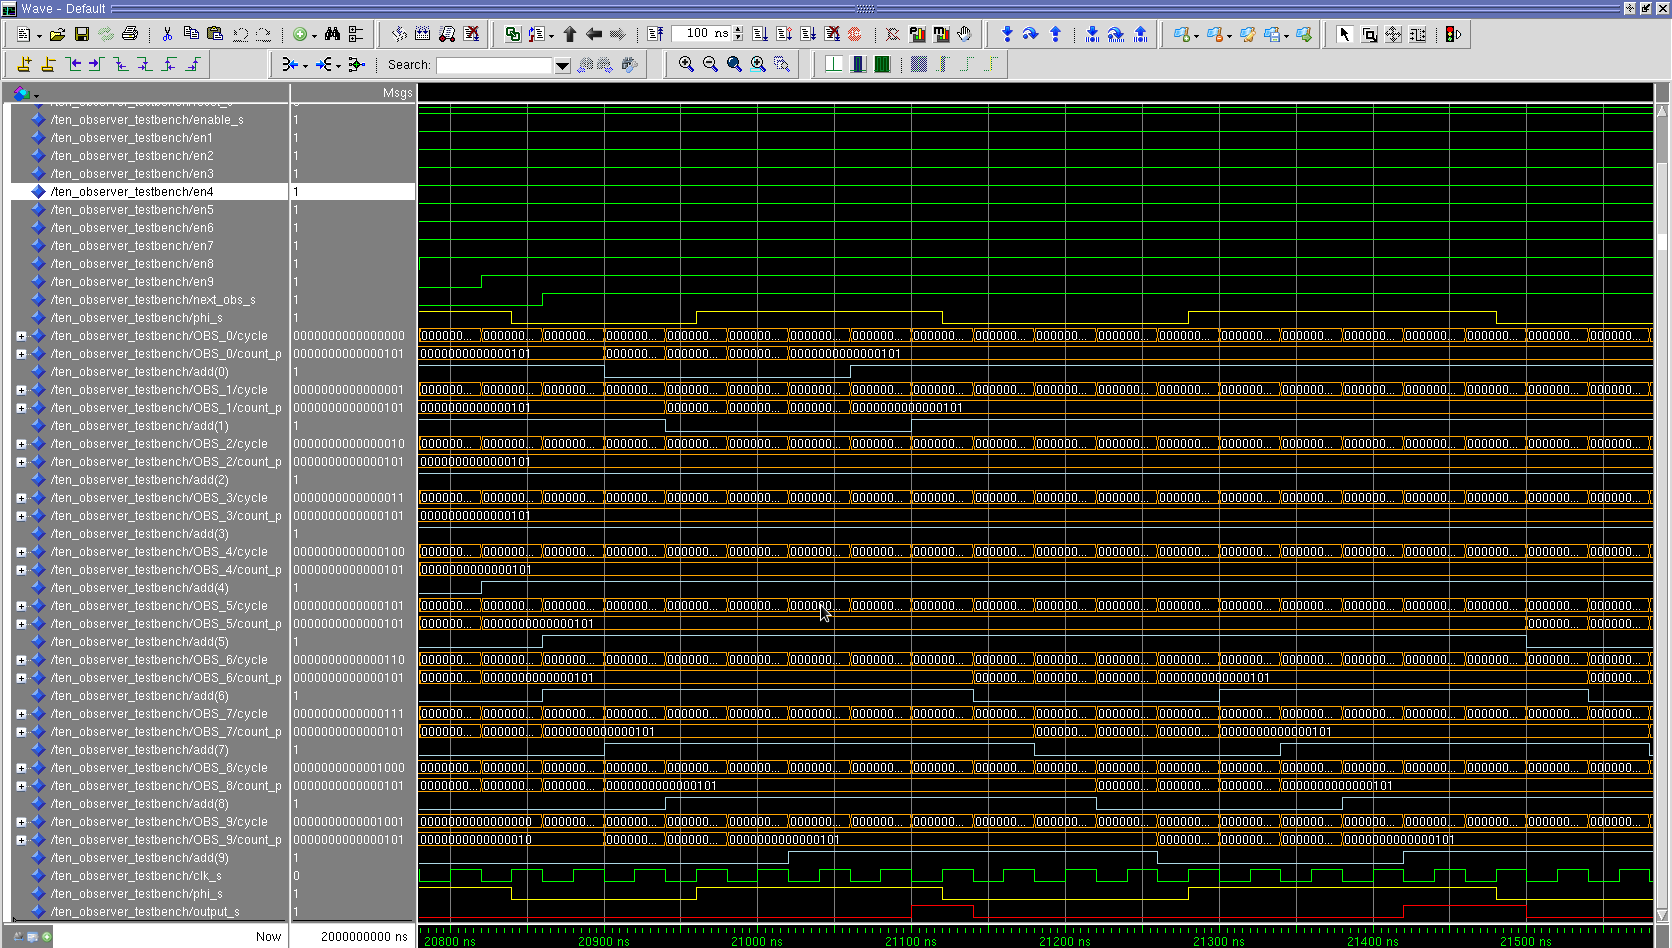
\includegraphics[width=650px,height=300px,angle=-90]{../../pictures/Modelsim/10_Observer_tb_2.png}
%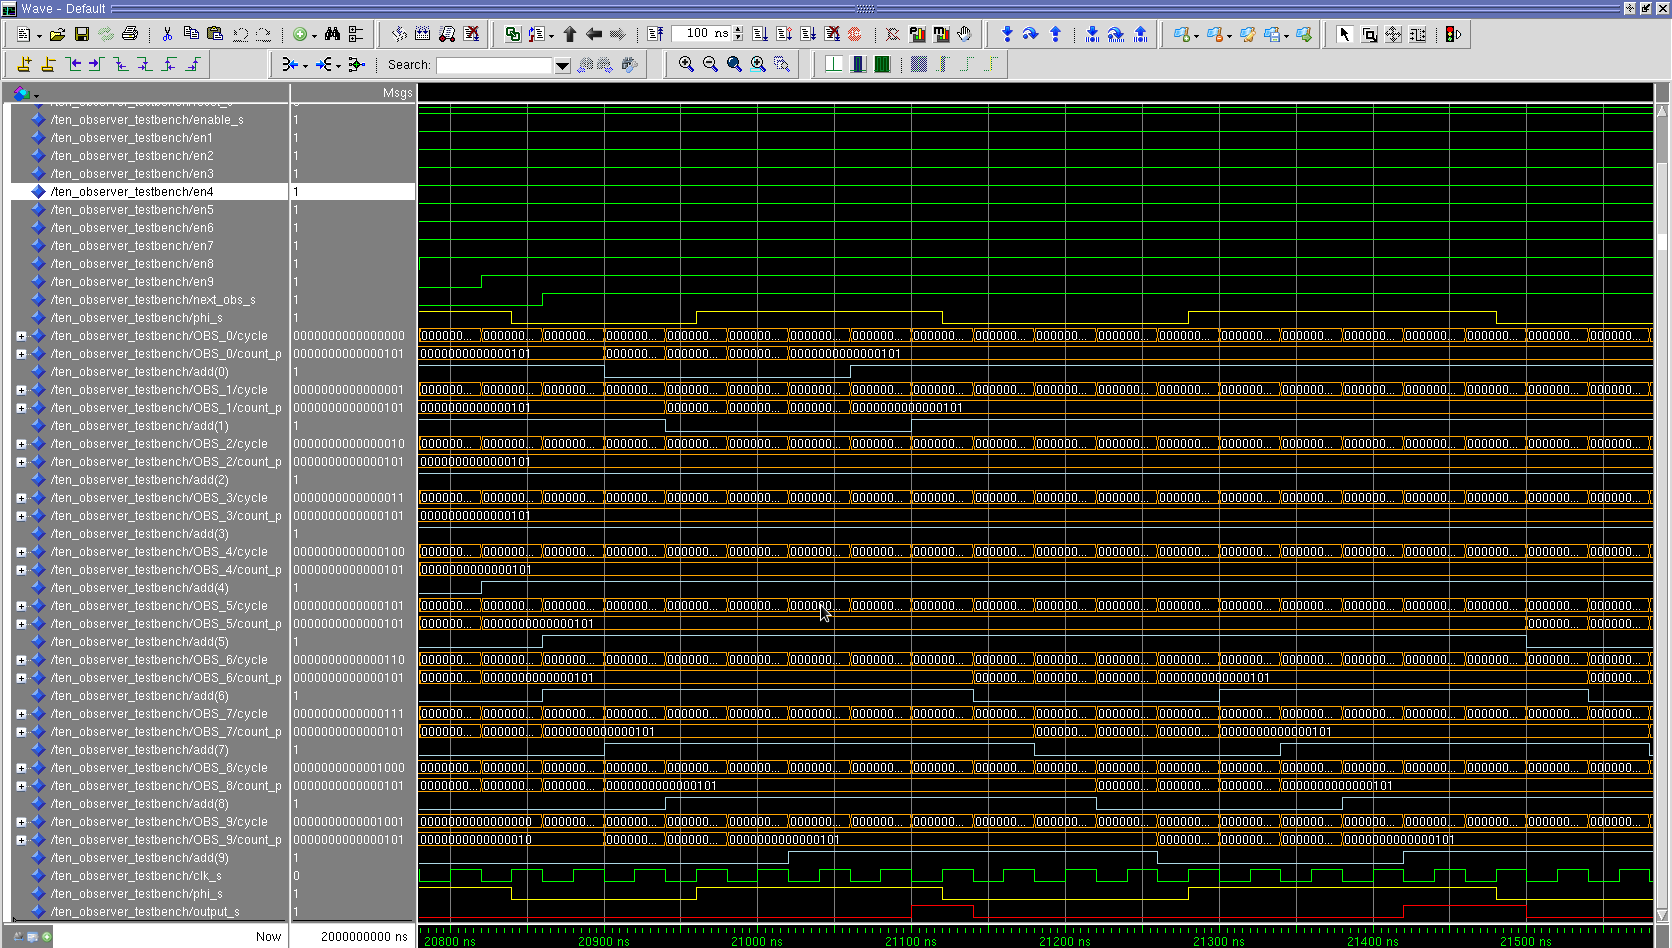
\includegraphics[height]{../../pictures/Modelsim/10_Observer_tb_2.png}
\caption[Modelsim Simulation of 10 Observer - 2]{m=10 Observer and $\tau=3$ with view about the output of the Observer Stages and final red-colored output}
\label{fig:simulation:ten:second}
\end{figure}

\begin{figure}[h]
\centering
%\hspace{3.0cm}
%\vspace{-5cm}
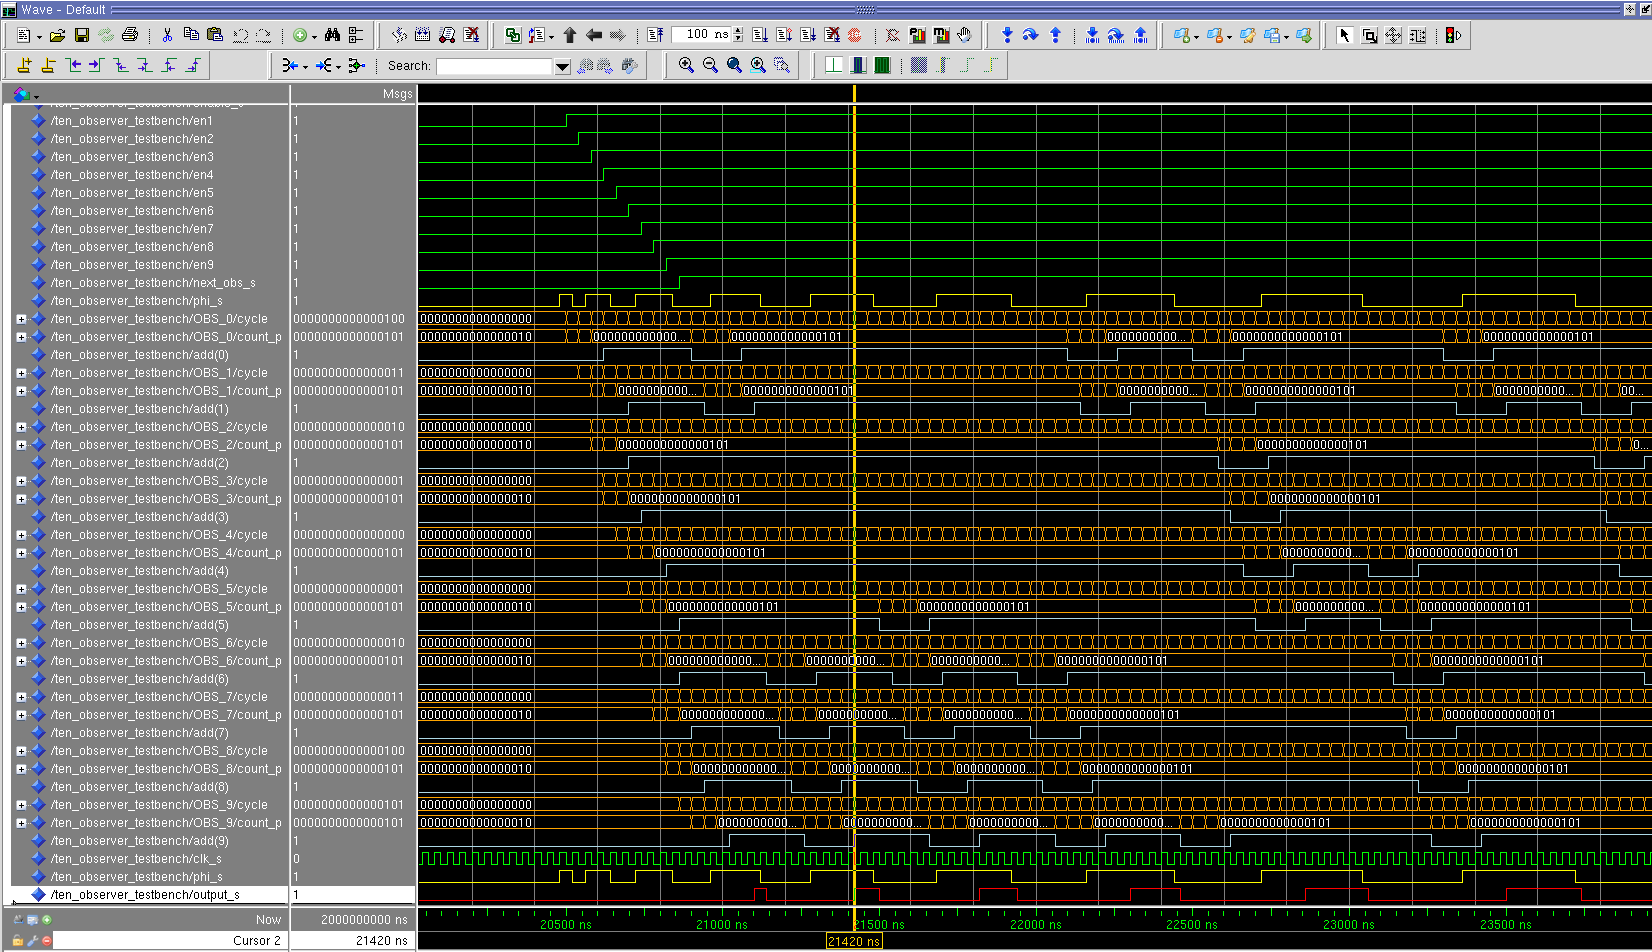
\includegraphics[width=650px,height=300px,angle=-90]{../../pictures/Modelsim/10_Observer_tb_3.png}
%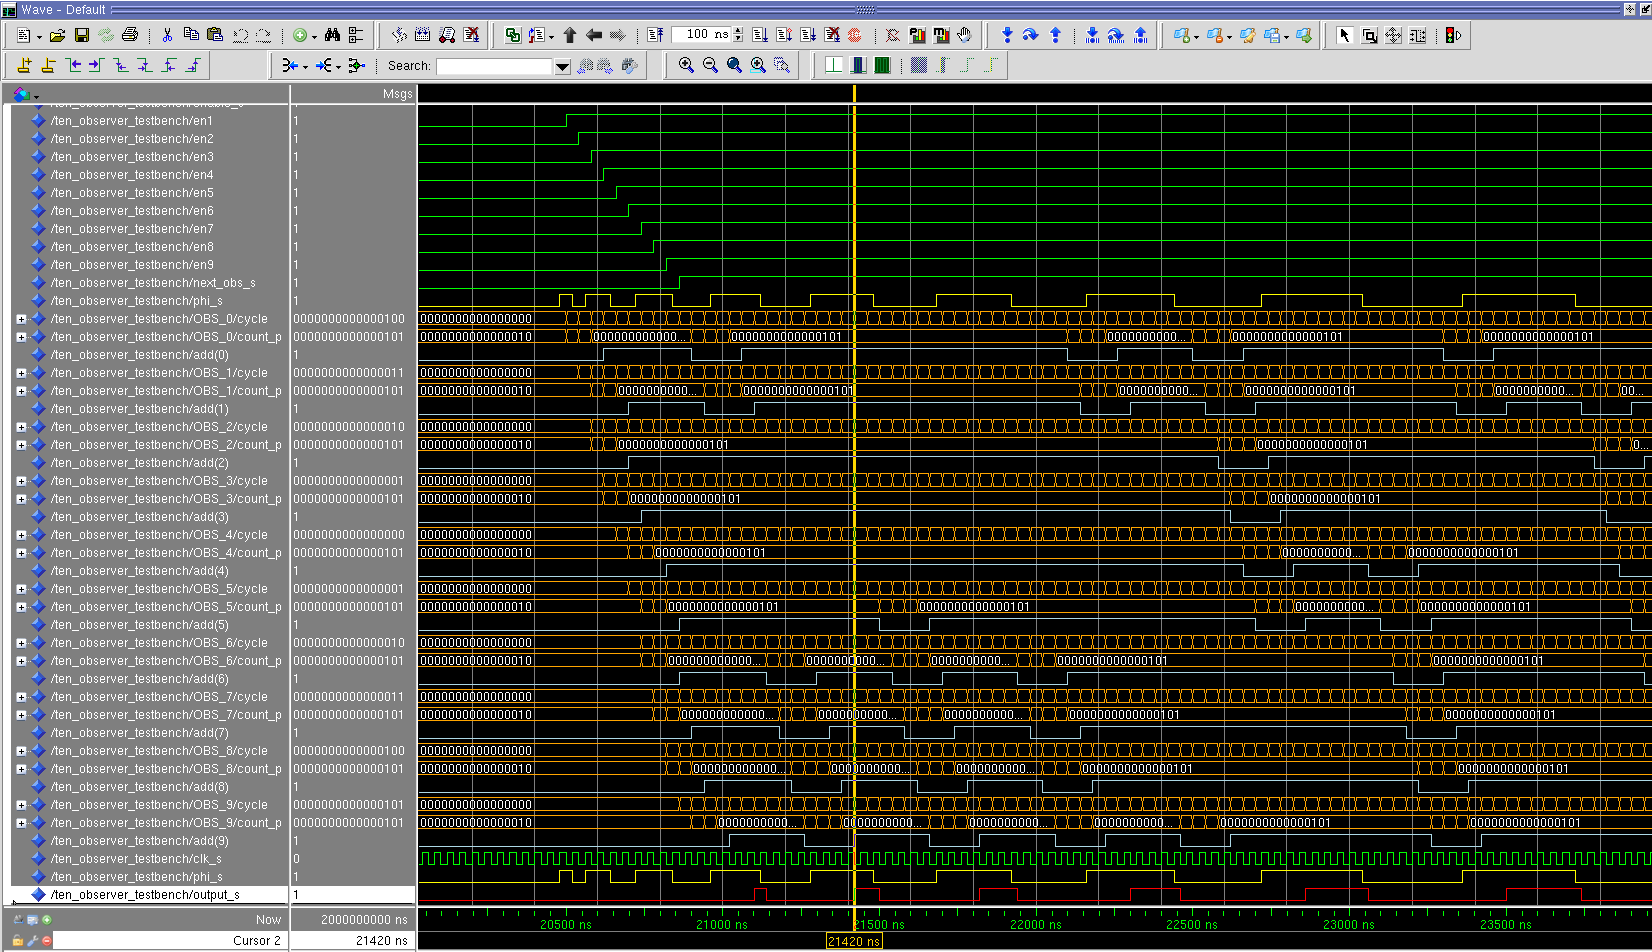
\includegraphics[height]{../../pictures/Modelsim/10_Observer_tb_3.png}
\caption[Modelsim Simulation of 10 Observer - 3]{m=10 Observer and $\tau=3$ with an overall view}
\label{fig:simulation:ten:third}
\end{figure}
